%%%%%%%%%%%%%%%%%%%%%%%%%%%%%%%%%%%%%%%%%%%%%%%%%%%%%%%%%%%%%%%%%%%
%                                                                 %
%                            CHAPTER                              %
%                                                                 %
%%%%%%%%%%%%%%%%%%%%%%%%%%%%%%%%%%%%%%%%%%%%%%%%%%%%%%%%%%%%%%%%%%%

\NewDocumentCommand{\codeword}{v}{%
\texttt{\textcolor{blue}{#1}}%
}

\DeclarePairedDelimiter\floor{\lfloor}{\rfloor}

\chapter{Implementation}
In this chapter we will explain how we implemented MPC for face matching algorithms. We will do this by giving a high-level overview of the system and then diving deeper in more interesting parts. With this information and the code in the appendix, you should be able to reproduce our experiments. You can also checkout our Github repository\footnote{\url{github.com/Fluxmux/securefacematching}}.
%TODO: Phrase this better

\section{Specifications}
There are two major subprojects. The first subproject (chapter \ref{Deep Learning}) is making sure we can generate the appropriate parameters for the face matching network. It is important that the model is accurate enough. The second subproject (chapter \ref{Secure Functions}) is about transforming the classic machine learning functions to secure ones. To add this security or privacy-preserving factor we use a MPC framework.

\subsection{Deep Learning}
\label{Deep Learning}
A machine learning project usually includes on of the popular frameworks available to the public. Since we were already familiar with Pytorch we used this library as a python package.

Pytorch \footnote{\url{pytorch.org}} provides us with a deep learning research platform that provides maximum flexibility and speed. It's fairly easy to use but that doesn't mean we can't design more complex models or features. Pytorch uses tensors, tensors are multi-dimensional matrix containing elements of a single data type. Designing a neural network with Pytorch is as simple as defining a class with the layers in the correct order. An example of a neural network written using pytorch can be seen in the following code (listing~\ref{lst:pytorch_example})\\

\begin{lstlisting}[language=Python, caption={Pytorch neural network example}, label={lst:pytorch_example}, frame=single]
class SiameseNetwork(nn.Module):
    def __init__(self):
        super(SiameseNetwork, self).__init__()

        self.cnn = nn.Sequential(
            nn.ReflectionPad2d(1),
            nn.Conv2d(1, 16, kernel_size=5),
            nn.ReLU(inplace=True),
            nn.BatchNorm2d(16),
            nn.MaxPool2d(kernel_size=2, stride=2),
            ...
        )
\end{lstlisting}

Making an accurate face matching neural network. Is a process that involves three major steps.

First of all the design or architecture of the network gets chosen. There exist a number of different topologies used in deep neural networks. But often choosing which one to take and how many layers to use, is the most difficult task. We will cover the architecture of the model in chapter \ref{ConvolutionalNeuralNetworkArchitecture}. Adding more layers is the same as adding more parameters. And a model with more parameters is more complex.

The second step is called the traing of the neural network. Training is done using a part of the dataset that is specific for training and shouldn't be used for anything else.

A typical workflow of the training step looks something like this: Two labeled faces are sent seperatly sent through the network. The euclidean distance (equation \ref{eq:euclideandistance}) for inputs $\vec{X_{1}}$ and $\vec{X_{2}}$ and the parameterized function $G_{W}$ calculates the distance between the outputs. This distance metric should be close to zero for faces belonging to the same person. But as large as possible for faces belonging to different person.

\begin{equation} \label{eq:euclideandistance}
  D_{W}(\vec{X_{1}},\vec{X_{2}})=\lVert G_{W}(\vec{X_{1}}) - G_{W}(\vec{X_{2}}) \rVert
\end{equation}

Then we use the loss function Yann LeCun first introduced in his paper \cite{hadsell2006dimensionality}; The general loss function $L$ is the sum of contrastive loss functions for a training pair in the set of training pairs of size $P$.

Let $Y$ be the binary label assigned to this pair of faces, $Y=0$ if $\vec{X_{1}}$ and $\vec{X_{2}}$ are labeled as similar, and $Y=1$ if $\vec{X_{1}}$ and $\vec{X_{2}}$ are labeled as dissimilar.

\begin{equation} \label{eq:contrastiveloss}
  L(W,Y,\vec{X_{1}},\vec{X_{2}})=(1-Y)\frac{1}{2}(D_{W})^{2} + Y\frac{1}{2}(max^{2}(0, m - D_{W}))
\end{equation}

The contrastive loss function is definded in formula \ref{eq:contrastiveloss}, where $m > 0$ is the margin. The margin $m$ can be seen as a radius so that dissimilar pairs still contribute to the loss function if their distance is withing this radius. The goal of training is to minimize the loss. For similar pairs this means decreasing the distance $D_{W}$, for dissimilar pairs this means increasing the distance to be greater than the margin. We came to the conclusion that our loss reduces the most if we choose a margin of $m=2$.

We also tried a different approach, instead of using this distance metric (which we would than have to statically threshold) we would like to have a probability value between $0$ and $1$. The output layer of the network consists out of two neurons (two classes), one neuron describes the similar faces, the other neuron describes the dissimilar faces. A probability of $0$ means that the faces belong to different persons and a probability of $1$ means that the faces belong to the same person. Binary Cross Entropy loss, or Logaritmic loss (equation \ref{eq:crossentropyloss}) is one of the loss functions that can be used to achieve this.

\begin{equation} \label{eq:crossentropyloss}
  L=-{(y\log(p) + (1 - y)\log(1 - p))}
\end{equation}

Let $y$ be the binary label assigned to this pair of faces, $p$ is the predicted probability. To visualize this loss function, have a look at figure \ref{fig:crossentropyloss}

\begin{figure}[H]
  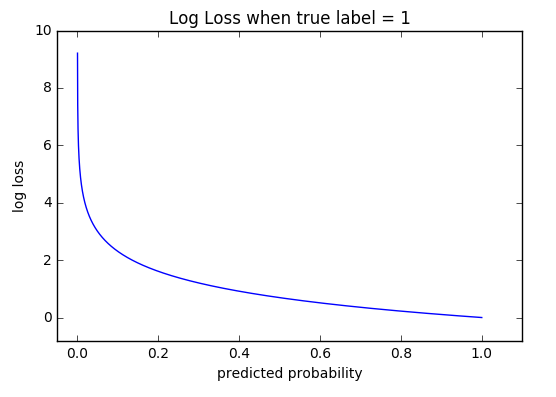
\includegraphics[scale=0.6]{fig/cross_entropy.png}
  \centering
  \caption{Range of loss values for $y=1$}
  \label{fig:crossentropyloss}
\end{figure}

There exist a great number of other functions. Some might be better suited for the face matching problem. But since we need to keep things simple in order to implement MPC. We opt for one of the two loss functions described above.

Training a neural network takes some time, but the process can be sped up by using graphics processing units (GPU). We were lucky enough to have a dedicated GPU server at our disposal. While training the network is an easy task, we should look out for overfitting or underfitting.

Overfitting a model happens when there are too much parameters for a model or when the training was performed for too long. It will perform poorly on the validation dataset (part of dataset used to detect bad trainig behaviour) while performing excellent on the training dataset. There are two ways of overcoming overfitting. One way is to make the training dataset larger. Having more samples to train on, generalizes the learning model better. The other way is to design the model with fewer parameters, making it less complex. We use learning curves to track the training process of our face matching algortihm. An example of a more or less correct learning curve can be found in figure \ref{fig:trainingcurve}.

\begin{figure}[H]
  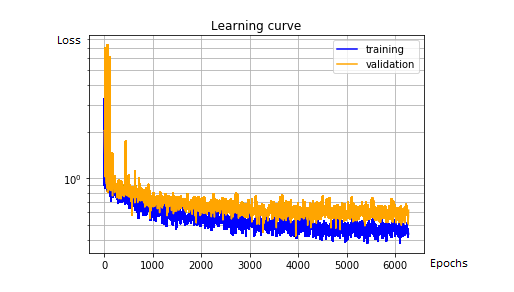
\includegraphics{fig/trainingcurve.png}
  \caption{Learning curves are used to track the training of a model}
  \label{fig:trainingcurve}
\end{figure}

Underfitting happens when a machine learning algorithm cannot capture the underlying structure of data. The model can't fit the data enough. Underfitting is more difficult to spot but easier to overcome. We can overcome this problem by making our model more complex.

As you can see by now, the architecture of a model is extremely important for it to function as wished.

The third step also called the hyperparameter tuning or hyperparameter optimisation step, is what makes a good machine learning model even better. This process is not at all logic, experience and intuition can facilitate this. Hyperparameters are all the parameters whose values are set before the learning process begins. There are different methods for optimizing hyperparameters, since we wanted to learn the model and how it behaves relating to small changes in the values of the hyperparameters we went for Manual Random Search. Note that this took us some time because this involves multiple training steps. But since we had a GPU server at our disposal we could parallelize this task. In our case this step improved our accuracy by about 5\%.

We used the Database of Faces\footnote{\url{cam-orl.co.uk/facedatabase.html}} to train and test our face matching algortihm. The dataset contains a set of 10 images of frontal faces with different expressions per person and a total of 40 persons. The pictures are in pgm format which is extremely easy to interact with. They have a dimension of 1 x 92 x 112. An example of a set of images from the dataset can be seen in figure \ref{fig:databaseoffaces}. We divided the dataset in to 3 parts: 75\% training, 12.5\% testing and another 12.5\% for validation.

\begin{figure}[H]
  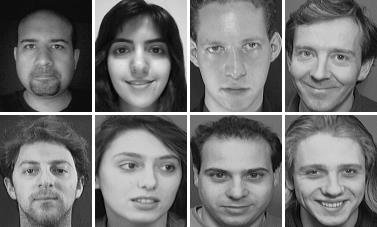
\includegraphics[scale=0.7]{fig/databaseoffacess.png}
  \centering
  \caption{Example of faces in dataset}
  \label{fig:databaseoffaces}
\end{figure}

\subsection{Secure Functions}
\label{Secure Functions}
Secure functions or the privacy preserving equivalent of an ordinary function can be used to compute an encrypted output as a function of encrypted inputs (figure \ref{fig:blackbox}). The protocol used for defining these secure functions is the MPC protocol.

\begin{figure}[H]
  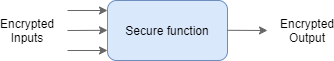
\includegraphics[scale=0.8]{plots/blackbox.png}
  \centering
  \caption{Secure function as a black box}
  \label{fig:blackbox}
\end{figure}

Berry Schoenmakers is a cryptographer working on cryptographic protocols for electronic voting, electronic payments and secure multiparty computation. Since 2018 he has been working on a general MPC implementation for python, called MPyC. This pyhton package can be easily installed with pip: \codeword{pip install mpyc}. The mpyc package defines two new number representation types: SecFxp and SecInt. SecFxp are secure fixed-point numbers. SecInt are secure integers. For more information on how to use this package have a look at the source code at \url{github.com/lschoe/mpyc}.

There are number of basic functions predefined, like \codeword{add}, \codeword{sub}, \codeword{mul} and \codeword{div}, respectively $+$, $-$, $\times$ and $\div$. As well as \codeword{eq} (equal to), \codeword{ge} (greater than or equal), \codeword{min} and \codeword{max}. The total set of available functions can be found in \codeword{mpyc.runtime.py}. But for our task the functions noted above are all we need.

With this set of fundamental functions we can generate our own custom functions that serve our needs.

\subsubsection{Custom Operations}

We introduce three essential custom secure functions that can be found in \codeword{custom_operations.py}.

\begin{itemize}
  \item \codeword{convolution}
  \item \codeword{maxpooling}
  \item \codeword{relu}
\end{itemize}

\codeword{convolution} is a secure function that takes two arguments $X$ and $W$ as input as can be seen in listing~\ref{lst:convolution}. Let $W$ be the kernel and $X$ the image over which to do the convolution. $X$ can be of any shape $(m, n)$, $W$ needs to be a square matrix of size $s$. We then define $Y$ to be the output matrix of the convolution function. Because the convolution is padded, $Y$ is of the same size as $X$.

\begin{lstlisting}[language=Python, caption={Secure convolution function}, label={lst:convolution}, frame=single, breaklines=true]
def convolution(X, W):
    m, n = dim(X)
    s = len(W)
    s2 = (s - 1) // 2
    Y = [None] * m
    for i in range(m):
        Y[i] = [None] * n
        for j in range(n):
            t = 0
            ix = i - s2
            for di in range(s):
                if 0 <= ix < m:
                    jx = j - s2
                    for dj in range(s):
                        if 0 <= jx < n:
                            t += X[ix][jx] * W[di][dj]
                        jx += 1
                ix += 1
            Y[i][j] = t
    return Y
\end{lstlisting}

Note that the number representation types that will be used in this secure convolution function, are not simple integers or floats. $X$, $W$ and $Y$ are matrices of SecInt's or SecFxp's.\\

\codeword{maxpooling} is a secure function (listing~\ref{lst:maxpooling}). The function takes one argument as input, $X$ an image of size $(m,n)$. We define a specific type of maxpooling, the pooling window has a size of $2$ by $2$ and the stride is equal to $2$. The output $Y$ is a matrix of size $(\floor*{\frac{m}{2}}, \floor*{\frac{n}{2}})$.

\begin{lstlisting}[language=Python, caption={Secure maxpooling function}, label={lst:maxpooling}, frame=single, breaklines=true]
def maxpool(X):
    m, n = dim(X)
    Y = [None] * (m // 2)
    for i in range(0, m - 1, 2):
        Y[int(i/2)] = [None] * (n // 2)
        for j in range(0, n - 1, 2):
            Y[int(i/2)][int(j/2)] = mpc.max(X[i][j], X[i][j+1], X[i+1][j], X[i+1][j+1])
    return np.array(Y)
\end{lstlisting}

\codeword{relu} is a secure function (listing~\ref{lst:relu}). The function takes one argument as input, $X$ the image of size $(m,n)$. This function doesn't change the shape of the input matrix, only the value of the elements of the matrix are changed, if they fulfill the condition.

\begin{lstlisting}[language=Python, caption={Secure ReLU function}, label={lst:relu}, frame=single, breaklines=true]
def relu(X):
    return np.vectorize(lambda a: (a >= 0) * a)(X)
\end{lstlisting}

Note that writing \codeword{a >= 0} or \codeword{mpc.ge(a, 0)} has the same effect. The same can be said for \codeword{(a >= 0) * a} and \codeword{mpc.mul(a >=0, a)}. The MPC operators are wrapped for the basic python operators on SecInt's and SecFxp's.\\

These three basic building blocks are essential for a convolutional neural network. But for the MPC protocol to function properly, we need to address some other problems. We will continue by giving a practical overview of the whole MPC protocol.\\

\begin{figure}[H]
  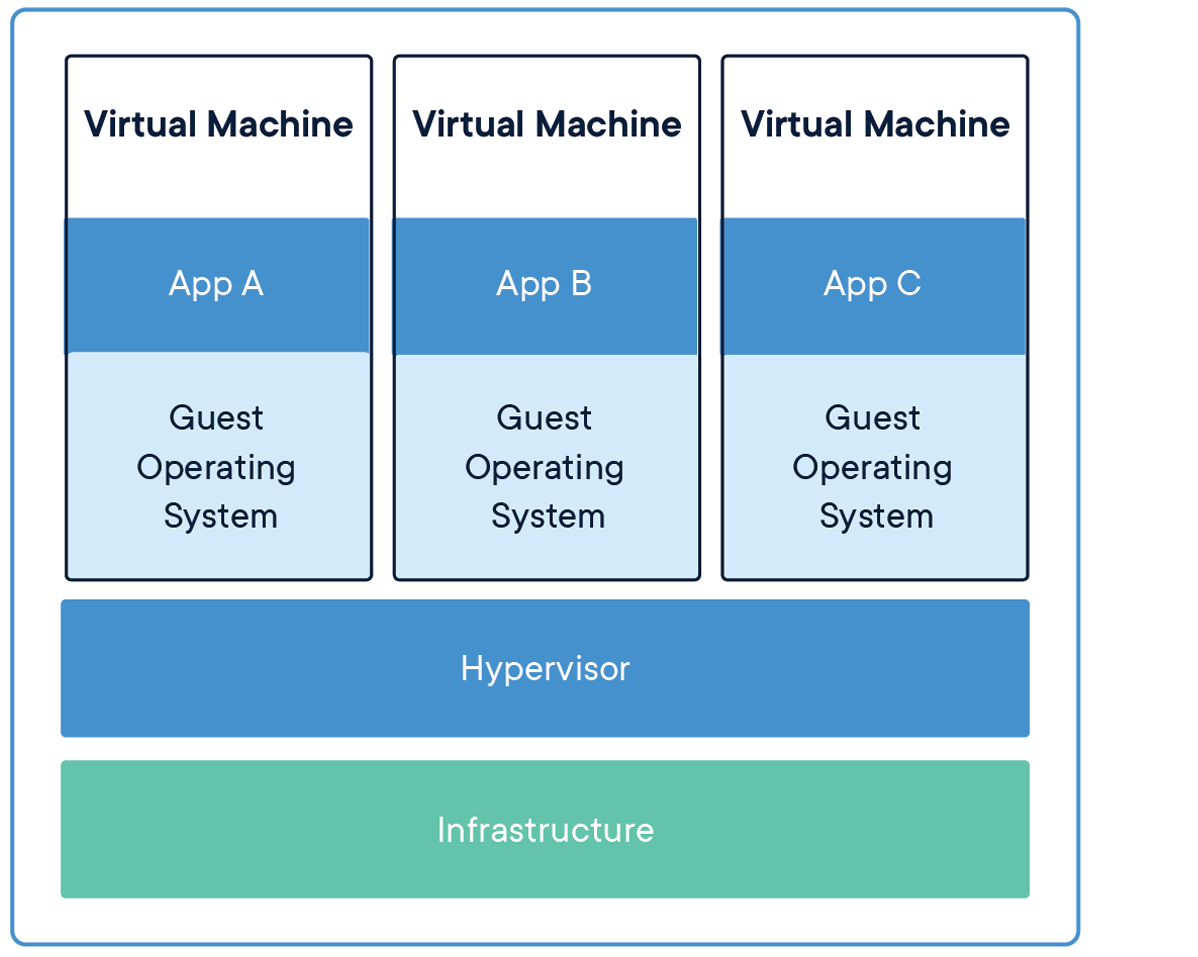
\includegraphics[scale=0.25]{fig/dockercontainer.png}
  \centering
  \caption{Three docker containers sharing the same infrastructure}
  \label{fig:dockercontainer}
\end{figure}

Suppose we have one user (device) and three computing parties (server)\footnote{Note that for ease, we use a loopback interface (localhost)}. We use the terms device and server to differentiate between two groups. On one hand we have the users who request a secure face matching task to be done, these users belong to the device group. On the other hand we have the parties doing the MPC, they belong to the server group.

The parties can be simulated by using three different Docker containers (figure \ref{fig:dockercontainer}), these containers share the same infrastructure (network). By setting the containers to different ports (5000, 5001, 5002 and 11365, 11366, 11367) on this network we can access, the containers from outside (device)\footnote{With outside we mean outside of the other containers, but the machine accessing the containers must still be on the loopback interface}. The Docker file (listing~\ref{lst:docker}) and environment file (listing~\ref{lst:env}) for  setting up the three parties.

\begin{lstlisting}[caption={Docker files for servers}, label={lst:docker}, frame=single]
FROM tsutomu7/scientific-python
MAINTAINER Carlton Shepherd "carlton.shepherd@onespan.com"
COPY . /app

# Install requirements
WORKDIR /app
RUN pip install -r requirements.txt

# Install MPyC from source after giving
# default user (scientist) all ownership
WORKDIR ./mpyc
USER root
RUN chown -R scientist .
USER scientist
RUN python setup.py install --user

#EXPOSE 11365

# Launch server
WORKDIR ../
CMD ["python -u", "./app.py"]
\end{lstlisting}

The \codeword{app.py} script runs a webserver using the python package flask and a database using the python package pymongo (MongoDB). The webserver will be used to communicate between the device and the server (to launch the MPC protocol, clear the database, ...) while the MongoDB will be used to store the secret shares for that particular server.

\begin{lstlisting}[caption={Environment file for servers}, label={lst:env}, frame=single]
N_PARTIES=3
PARTY_0_HOST=localhost
PARTY_0_PORT=5000
PARTY_1_HOST=localhost
PARTY_1_PORT=5001
PARTY_2_HOST=localhost
PARTY_2_PORT=5002
\end{lstlisting}

When all three parties (server) are up and running, the user (device) can start encrypting their input image containing their face using Shamir's secret sharing scheme (listing \ref{lst:ssss}). The user shares each pixel of the image in to three secret shares, one for each party. The user then sends their three sets of secret shares (encrypted image) to the parties, each party receives only one set of shares.

\begin{lstlisting}[caption={Shamir secret sharing algorithm}, label={lst:ssss}, frame=single, breaklines=true]
def random_split(s, t, m):
    field = type(s[0])
    p = field.modulus
    order = field.order
    T = type(p) # T is int or gf2x.Polynomial
    n = len(s)
    shares = [[None] * n for _ in range(m)]
    for h in range(n):
        c = [secrets.randbelow(order) for _ in range(t)]
        # polynomial f(x) = s[h] + c[t-1] x + c[t-2] x^2 + ... + c[0] x^t
        for i in range(m):
            y = 0 if T is int else T(0)
            for c_j in c:
                y += c_j
                y *= i + 1
            shares[i][h] = (y + s[h].value) % p
    return shares
\end{lstlisting}

The algorithm above splits each secret given by parameter s (list of secrets) into m random Shamir shares. The degree for the Shamir polynomials is t remember  $0 \leq t < n$. The algorithm returns a matrix of shares, one row per party.\\

Finally the user can start the computation by, sending a the appropriate request to one of the parties (listing \ref{lst:devicelaunch}). We make use of the requests package, requests is a simple HTTP library for python it enables us to make requests and get responses over HTTP.

\begin{lstlisting}[caption={Sending request for secure face matching task}, label={lst:devicelaunch}, frame=single, breaklines=true]
# Define hosts and ports
hosts = ['localhost', 'localhost', 'localhost']
ports = [5000, 5001, 5002]

# Shares secrets
image = cv2.imeread("face.pgm")
kernel = [[1,1,1],[0,0,0],[-1,-1,-1]]
send_shares_mpc(image, ['Image'], 'test', hosts, ports, combined = True)
send_shares_mpc(kernel, ['Filters'], 'model', hosts, ports, combined = True)

# Start MPC
url = f'http://{hosts[0]}:{ports[0]}/mpyc_launch?api=face_matching_server'
response = requests.get(url)
# Response contains output of the MPC
\end{lstlisting}

Note that the HTTP response we get from the GET request contains two variables; the status code and the text. The status code indicates wheter the HTTP request has been  succesfully completed, a valid and succesfull request has a response code of 200. The text of a response is the message that is transferred in the body of the HTTP response. We use the HTTP as means of communication between the device and the server. Note that for more secure implementations, HTTPS (Hypertext Transfer Protocol Secure) is preferred. Since traffic in HTTPS is encrypted using Transport Layer Security (TLS). Using HTTPS denies MITM attacks (man-in-the-middle), a type of attack where a passive attacker tries to eavesdrop certain packets of the traffic.\\

The GET query of the request sent in listing \ref{lst:devicelaunch} executes the following code (listing \ref{lst:mpyclaunch}) on the first party or PARTY\_0 (localhost:5000).

\begin{lstlisting}[caption={Launching MPC and returning formatted output}, label={lst:mpyclaunch}, frame=single, breaklines=true]
is_running = False
@app.route("/mpyc_launch", methods=["GET"])
def mpyc_launch():

    def get_api_name(api_name):
        return api_name + '.py'

    http_arg = request.args.get('api')
    script_name = get_api_name(http_arg)
    if script_name is None:
        return "400"

    os.chdir(main_wd)
    test_path="./mpyc/demos"
    os.chdir(test_path)
    # Raise other parties
    Party = os.getenv(f"Party")
    # Only execute following code for PARTY_0
    if Party == '0':
        global is_running
        if is_running:
            return '200'
        else:
            is_running = True

        for i in range(int(os.getenv('N_PARTIES')) - 1, 0, -1):
            party_host = os.getenv(f'PARTY_{i}_HOST')
            party_port = os.getenv(f'PARTY_{i}_PORT')
            host_addr = f'http://{party_host}:{party_port}/mpyc_launch?api={http_arg}'
            r = requests.get(host_addr)
            time.sleep(2.50)

        # Run MPC script (PARTY_0)
        process = subprocess.Popen(['python', script_name, '-c', f'party{3}_0.ini'], stdout=subprocess.PIPE)
        stdout, stderr = process.communicate()
        is_running = False

        # Output everything inside of the '$$$' tags
        output_formatted = stdout.decode().split('$$$')[1]
        output_formatted = output_formatted.split('$$$')[0]
        output_formatted = output_formatted.strip()
        output_formatted = output_formatted.replace('\n', '')
        output_formatted = output_formatted.strip(',')
        return output_formatted

    else:
        # Run MPC script (party_1 and party_2)
        os.system(f'python {script_name} -c party{3}_{Party}.ini &')
        return "200"
\end{lstlisting}

The value of the api argument from the GET request determines which MPC script gets excecuted. Then PARTY\_0 starts executing the same code snippet (mpyc\_launch) on the other two parties, by sending the appropriate requests. The first party then executes a new subprocess that runs a the MPC script. The result of the MPC script gets written to the STDOUT stream (standard output) which can be read by the parent process. The result gets parsed in the MPC script, by printing the result between two \$\$\$ tags (like this \$\$\$ result \$\$\$). The other two parties skip most of the code (because their environment variable 'Party' differs from 0) and go straight to executing the same MPC script. Notice that PARTY\_0 plays an important role in establishing that the MPC script runs on the other parties. This centralisation is a clear weakness of this implementation, because a corrupted PARTY\_0 could cause great harm to the correctness of the protocol. But for the sake of simplicity we opt for this more centralised implementation. An overview of this implementation with the different groups (device and server) can be seen in figure \ref{fig:implementationoverview}.

\begin{figure}[H]
  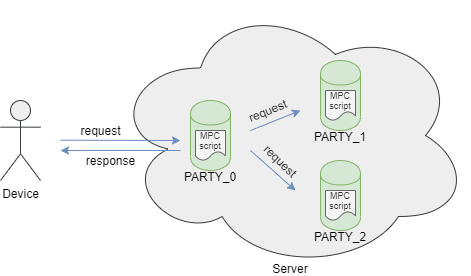
\includegraphics[scale=0.75]{fig/implementationoverview.png}
  \centering
  \caption{Overview of MPC implementation over HTTP (3 parties)}
  \label{fig:implementationoverview}
\end{figure}

Last but not least, we discuss the mpc script that needs to run on the three parties. This script does the actual MPC. Each party holds an identical copy of this script. The parties begin by opening connections with each other (\codeword{mpc.start}). Remember: parties need to communicate with each other in order to output a result or to do non-linear operations such as multiplication of two secure numbers. Then the parties load the unique secret shares for the image and the convolution kernels stored in their MongoDB databases. Since the secret shares are stored in lists in the database, the parties reshape them to the original shape. Then the parties securely compute an output for the input image and kernels on a series of sequential layers (convolution, maxpooling and relu) made out of the essential building blocks we introduced at the beginning of this chapter. Finally the parties output the result (\codeword{mpc.output}) print the result (printing in python has the same effect as writing to STDOUT) but they do this in a manner such that the stream is parsed. Note that all parties print the result, but only PARTY\_0's STDOUT will be looked at. This is yet another flaw of our implementation. Better would be to look at everybody's STDOUT, to check if anyone is cheating by printing something other than the true result. Finally the parties begin shutting down (mpc.shutdown), closing all open connections. The subprocess will exit, unpausing the parent process. Which will unparse the STDOUT and return the result as a response to the device.\\

 A basic example of an mpc script that contains all of the points made earlier can be observed in listing \ref{lst:mpcscript}.

\begin{lstlisting}[caption={Example of MPC script for a single CNN layer (conv,maxp and relu)}, label={lst:mpcscript}, frame=single, breaklines=true]
import math
import numpy as np
from mpyc.runtime import mpc
from load_database import load_data
from custom_operations import convolution, relu, maxpool

async def main():
    await mpc.start()

    images = load_data('Image', 'test')
    kernels = load_data('Filters', 'model')
    image = images[0]
    kernel = kernels[0]

    image = np.reshape(image, (int(math.sqrt(len(image))), int(math.sqrt(len(image)))))
    kernel = np.reshape(kernel, (int(math.sqrt(len(kernel))), int(math.sqrt(len(kernel)))))

    conv = convolution(image, kernel)
    maxp = maxpool(conv)
    result = relu(maxp)
    result = list(np.asarray(result).flatten())

    print("$$$\n")
    print(await mpc.output(result))
    print("$$$")

if __name__ == '__main__':
    mpc.run(main())
\end{lstlisting}

Obviously a CNN has way more layers than just this triplet (convolution, maxpooling and relu). But we will discuss the secure design of the CNN later on in chapter \ref{SecureCNN}.

\section{Design}
\label{Design}
In this chapter we discuss how we designed the neural network and why we chose for the network's architecture in specific. After explaining the neural network's architecture, we will have a look at how we translate a model working on plaintext pictures, to a secure model using MPC.

\subsection{Convolutional Neural Network Architecture}
\label{ConvolutionalNeuralNetworkArchitecture}
In the process of choosing the best architecture for a CNN, we found four suitable models. We will see how each of these models are designed and in what way they differ from the others. Finally, we select one of these models to make it secure using MPC, the selection depends on the following criteria; straightforwardness of the MPC implementation, size of the network (number of parameters), accuracy of the model and the preferred output (distance vector or binary classification).\\

\textbf{General (applies for all models):} The input dimensions of the different neural networks is the same (1 x 100 x 100). The output can differ depending on what loss function is used (cross entropy loss or contrastive loss), but the meaning is the same, wheter a face matches another face or not. And the only difference is how to differentiate between these two classes (match or no match), this means the arbitrary threshold must be chosen on a different basis. To choose a good threshold that reflects the accuracy of the model, we iterate the calculation of the precision and recall for each threhold value in a certain range. This gets us the following curve (figure \ref{fig:threshold}), out of which we can distract the best threshold.\\

\begin{figure}[H]
  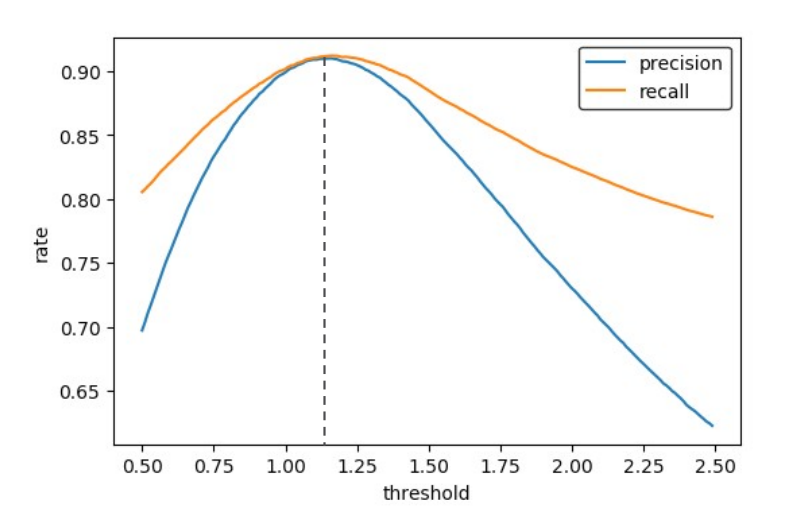
\includegraphics[scale=0.6]{fig/threshold.png}
  \centering
  \caption{Curve for selecting the best threshold value}
  \label{fig:threshold}
\end{figure}

\textbf{CNN with Contrastive Loss:} This model is the first model we designed. It is simple and basic yet powerful. The neural network design can be seen in figure \ref{fig:ccncl}.

\begin{figure}[H]
  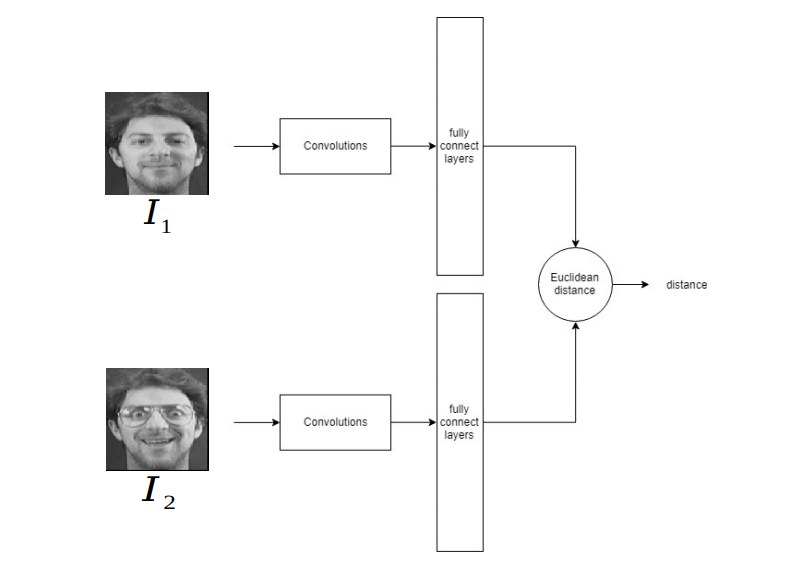
\includegraphics[scale=0.7]{fig/cnncl.png}
  \centering
  \caption{CNN with Contrastive Loss function}
  \label{fig:ccncl}
\end{figure}

The convolution layers, including Max-pooling (2 x 2 with stride 2) and ReLU after every convolution, consist out of four layers:

\begin{enumerate}
  \item 4 convolutions (7 x 7).
  \item 8 convolutions (5 x 5).
  \item 16 convolutions (3 x 3).
  \item 32 convolutions (3 x 3).
\end{enumerate}

Each of these layers have different tasks. The first layers have larger convolution filters, these convolutions detect high-level features like distance or rotation between ears, nose and/or eyes. While the latter, smaller convolution filters detect low-level features like lines or dots (jawline, eyes, mouth).

After the final convolution layer we flatten the output layer to a one-dimensional tensor. This tensor then serves as input for a small fully-connected neural network (perceptron), this network can be seen as an extension of the CNN. We use this fully-connected neural network to add global spatial correlation (a CNN is good for recognizing structures in local and neighbouring pixels). Since it's important to also important that the algorithm detects two objects or features that belong to each other even though they are seperated and are not local or neighbouring, think of two ears on a face for instance.\\

The total number of learnable parameters (weights and biases) in this neural network is 154.592, the model doesn't show any sign of overfitting nor underfitting up to 500 epochs.\\

The code for this neural network is printed in below (listing~\ref{lst:cnncl}). Notice how simple this neural network is. With only four convolutional layers, it is able to make a face matching decision.

\begin{lstlisting}[caption={Code for CNN with Contrastive Loss}, label={lst:cnncl}, frame=single, breaklines=true]
class SiameseNetwork(nn.Module):
    def __init__(self):
        super(SiameseNetwork, self).__init__()

        self.cnn1 = nn.Sequential(
            nn.Conv2d(1, 4, kernel_size=7),
            nn.MaxPool2d(kernel_size=2, stride=2, padding=0),
            nn.ReLU(),
            nn.Conv2d(4, 8, kernel_size=5),
            nn.MaxPool2d(kernel_size=2, stride=2, padding=0),
            nn.ReLU(),
            nn.Conv2d(8, 16, kernel_size=3),
            nn.MaxPool2d(kernel_size=2, stride=2, padding=0),
            nn.ReLU(),
            nn.Conv2d(16, 32, kernel_size=3),
            nn.MaxPool2d(kernel_size=2, stride=2, padding=0),
            nn.ReLU(),
        )

        self.fc1 = nn.Sequential(nn.Linear(512, 256), nn.ReLU(), nn.Linear(256, 64))

    def forward_once(self, x):
        output = self.cnn1(x)
        output = output.view(output.size()[0], -1)
        output = self.fc1(output)
        return output

    def forward(self, input1, input2):
        output1 = self.forward_once(input1)
        output2 = self.forward_once(input2)
        return output1, output2
\end{lstlisting}

\textbf{CNN with Cross Entropy Loss:} The following model (figure \ref{fig:cnncel}) is similar to the first one we described earlier. The key differences of this model, is that the siamese neural network stops after the last layer. The two output layers get flattened to two single one-dimensional tensors. These tensors then get concatenated. The concatenated tensor now gets sent trough a single fully-connected neural network (perceptron).\\

\begin{figure}[H]
  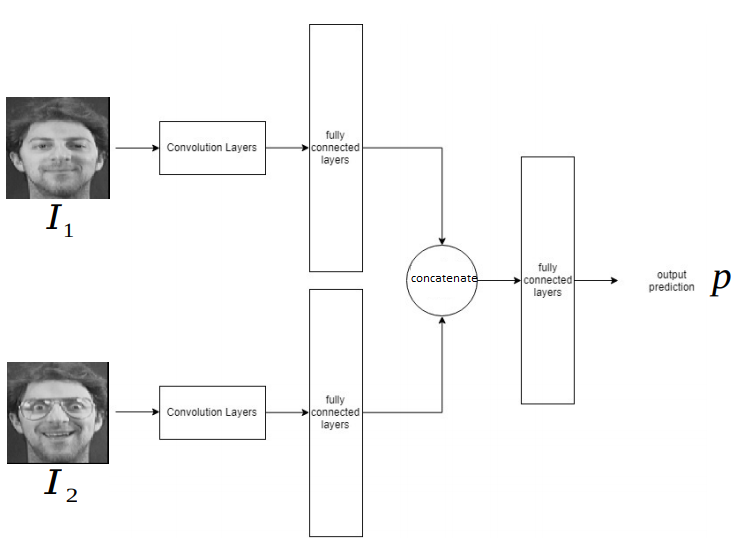
\includegraphics[scale=0.7]{fig/cnncel.png}
  \centering
  \caption{CNN with Cross Entropy Loss function}
  \label{fig:cnncel}
\end{figure}

 Note that in the first model (CNN with Contrastive Loss) there is no fusion of the siamese neural network. And the only time the two inputs depend on each other, is when we calculate the euclidean distance between the two output tensors. In fact, this type of model is not really a pure siamese neural network anymore. We guess that the perceptron, placed after the convolution layers, performs some sort of comparison on the two output tensors and we hope this comparison will be better than the standard euclidean distance.\\

 Finally, the cross entropy loss is calculated on the last layer of the model. Since face matching is a binary task (matching or not matching), the last layer contains a single neuron (class). The cross entropy of that neuron returns the chance for that class to be true. The pleasant advantage of cross entropy is that we don't have to set up an arbitrary threshold value, the threshold is simply already decided, for instance if $p \in [0,1]$ than the threshold is equal to $p = 0.5$. If two faces are simmilar, $p=0$. If two faces are dissimilar, $p=1$.\\

 The convolution layers consist of the same number of convolutions, as the first model:

 \begin{enumerate}
   \item 4 convolutions (7 x 7).
   \item 8 convolutions (5 x 5).
   \item 16 convolutions (3 x 3).
   \item 32 convolutions (3 x 3).
 \end{enumerate}

 The code for the model is listed below (listing~\ref{lst:cnncel})

 \begin{lstlisting}[caption={Code for CNN with Cross Entropy Loss}, label={lst:cnncel}, frame=single, breaklines=true]
 class SiameseNetworkConcat(nn.Module):
    def __init__(self):
        super(SiameseNetwork, self).__init__()

        self.cnn1 = nn.Sequential(
            nn.Conv2d(1, 4, kernel_size=7),
            nn.MaxPool2d(kernel_size=2, stride=2),
            nn.ReLU(),
            nn.Conv2d(4, 8, kernel_size=5),
            nn.MaxPool2d(kernel_size=2, stride=2),
            nn.ReLU(),
            nn.Conv2d(8, 16, kernel_size=3),
            nn.MaxPool2d(kernel_size=2, stride=2),
            nn.ReLU(),
            nn.Conv2d(16, 32, kernel_size=3),
            nn.MaxPool2d(kernel_size=2, stride=2),
            nn.ReLU(),
        )

        self.fc1 = nn.Sequential(
            nn.Linear(1600, 100), nn.ReLU(inplace=True), nn.Linear(100, 10),
        )

        self.fc2 = nn.Sequential(
            nn.Linear(20, 20), nn.ReLU(inplace=True), nn.Linear(20, 1),
        )

    def forward_once(self, x):
        output = self.cnn1(x)
        output = output.view(output.size()[0], -1)
        output = self.fc1(output)
        return output

    def forward(self, input1, input2):
        output1 = F.relu(self.forward_once(input1))
        output2 = F.relu(self.forward_once(input2))
        output = torch.cat((output1, output2), dim=1)
        output = self.fc2(output)
        return output
 \end{lstlisting}

\textbf{Residual Neural Network:} The last model make use of a special type of deep learning, known as deep residual learning, introduced in 2015 by \cite{he2016deep}. A Residual Neural Network (ResNet) is a special type of neural network that utilizes shortcuts or skip connections shortcuts to jump over a number of layers. Neural networks implementing residual blocks (figure \ref{fig:residualblock}) can have way more layers without running in to problems like vanishing gradient. Vanishing gradient problem occurs when certain parameters of a network do not get updated during training, because the gradient will be so small that it will prevent the parameters from changing. With ResNet a direct link (identy function) can be found over multiple layers, thus creating a way to link certain inputs deeper into the network.

\begin{figure}[H]
  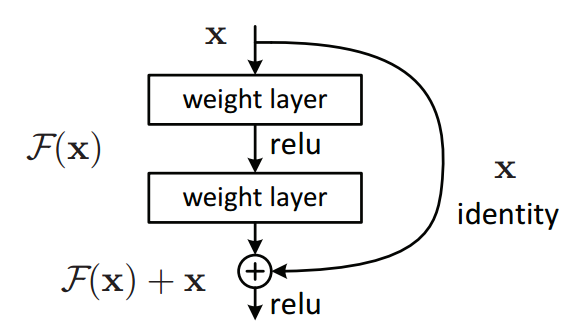
\includegraphics[scale=0.5]{fig/residualblock.png}
  \centering
  \caption{Residual block (2-layer skipping)}
  \label{fig:residualblock}
\end{figure}

In short, ResNet allows us to use way more layers than before. So we derived our own ResNet-like model, from the pre-trained ResNet models available from Pytorch \footnote{\url{github.com/pytorch/vision/blob/master/torchvision/models/resnet.py}}. We saw an incline in accuracy using ResNet, but with more layers, there are more parameters and the complexity rises.

A basic residual block can be coded in Pytorch in the following way (\ref{lst:residualblock})

\begin{lstlisting}[caption={Pytorch Code for Residual Block}, label={lst:residualblock}, frame=single, breaklines=true]
class BasicBlock(nn.Module):
    def __init__(self, in_planes, planes, stride=1):
        super(BasicBlock, self).__init__()
        self.expansion = 1
        self.conv1 = nn.Conv2d(in_planes, planes, kernel_size=3)
        self.bn1 = nn.BatchNorm2d(planes)
        self.conv2 = nn.Conv2d(planes, planes, kernel_size=3)
        self.bn2 = nn.BatchNorm2d(planes)
        self.pool = nn.MaxPool2d(2,2)

        self.shortcut = nn.Sequential()
        if stride != 1 or in_planes != self.expansion*planes:
            self.shortcut = nn.Sequential(
                nn.Conv2d(in_planes, self.expansion*planes, kernel_size=1, stride=stride, bias=False),
                nn.BatchNorm2d(self.expansion*planes)
            )

    def forward(self, x):
        out = F.dropout(F.relu(self.bn1(self.conv1(x))), p=0.3)
        out = self.bn2(self.conv2(out))
        out += self.shortcut(x)
        out = F.relu(out)
        return out
\end{lstlisting}

Notice that the \codeword{self.shortcut} function is simply the identity function.\\

As we said before choosing a neural network depends on a number of factors, we will now rank each of the neural networks described above for each determining factor.\\

Starting with the straightforwardness of the MPC implementation, in other words, how easy will it be to translate the code written with Pytorch to a MPC algorithm using no libraries for neural networks (since Pytorch doesn't support secure datatypes). It's obvious that a ResNet architecture requires more attention to detail and is more complex to implement. The other two neural networks require less attention to detail, thus are more easy to implement.\\

Next, we compare size of the neural network. The neural network's size or it's number of parameters is an equally important factor. Since MPC protocols are way slower than classic computations. We would like our neural network to do fast computations. Fast computations corresponds to less computations, and less computations corresponds to less (or smaller) convolutions or fully-connected layers. Thus we would like our network to have a small number of layers, but still enough to be able to differentiate between faces. Since ResNet only adds extra layers, this model is again not preffered. The other two models have about the same number of parameters, and only the fully-connected layers have a different number of weights and biases.\\

Ranking the neural networks on accuracy (the ability to match faces) was done by testing the four different networks, the results can be seen in table \ref{designaccuracy}. We find that when we are using the Contrastive Loss function, the classic CNN as well as the ResNet model is giving us better results than with the Cross Entropy loss function. Overall the ResNet model has a slightly better accuracy than the classic CNN.

\begin{table}[]
\begin{tabular}{llc}
\hline
\multicolumn{1}{|l|}{Model} & \multicolumn{1}{l|}{Loss} & \multicolumn{1}{l|}{Accuracy} \\ \hline
Classic CNN                 & Contrastive Loss          & 89.20\%                       \\
Classic CNN                 & Cross Entropy Loss        & 81.94\%                       \\
ResNet (8 layers)           & Contrastive Loss          & 91.06\%                       \\
ResNet (8 layers)           & Cross Entropy Loss        & 84.13\%
\end{tabular}
\caption{Accuracy of the different models}
\label{table:designaccuracy}
\end{table}

Last but not least, what output do we prefer? The models with Contrastive loss have an output in the form of a score, the distance between two output vectors gets calculated. While the models with Cross Entropy loss simply output a chance, not having to worry about choosing a certain threshold. During the testing of the networks we argued that determining the threshold is not too hard, in fact the threshold can be easily chosen by drawing out a graph of the accuracy of the network and the different thresholds as in figure \ref{fig:ccncl}.\\

Taking every factor in to consideration, we concluded that a classic CNN with Contrastive Loss offers a high enough accuracy and low complexity, while still being easy to implement in MPC.\\

In the following part of this chapter we will discuss specifically what parts of the classic CNN we will encrypt.

\subsection{Secure CNN}
\label{SecureCNN}


\section{Conclusion}
